\section{Results and discussion\label{sec:results_and_discussion}}
In this section, we present and discuss the results of the dimension analyses. We analyze the three dimensions \emph{performance}, \emph{privacy}, and \emph{complexity}. We commence with a qualitative and quantitative analysis of the \emph{performance} dimension and continue with qualitative analyses of the \emph{privacy} and \emph{complexity} dimensions.

\subsection{Performance analysis in the SME context}
As explained in section \ref{sec:methodology_study_setup} we distinguish four scenarios regarding the data and label distribution. In the following, we analyze and compare these four scenarios for the case of five clients taking part in the FL task. Results for fewer and more clients are presented in the appendix in sections \ref{sec:2_clients} and \ref{sec:10_clients}. In the \emph{one model per client} setting, each of these five clients trains its own model solely on its own data. In the \emph{all data model} setting, one model is trained on the union of the five clients' data. In the FL setting, these five clients take part in the learning task and train a joint model without sharing their data but only sharing parameters of their models via a central node.

\subsubsection{Analysis results\label{sec:analysis_results}}
\paragraph*{Balanced data distribution - balanced label distribution} In this scenario, the data and the label distribution between the five clients are balanced, meaning each client has the same amount of data and each of the five clients has as many ``pitting'' as ``no pitting'' images.
In this simulation, we expect all clients in the \emph{one model per client} setting to perform equally well, except for random performance differences due to the randomness introduced in the data split. We expect the \emph{all data model} to perform better than or equally well as the FL setting as both can leverage all the data, although the learning process might perform better in the \emph{all data model} setting, especially due to the optimizer. We will pick up this point in the discussion in section \ref{sec:discussion_performance} in detail.

In figure \ref{fig:auc_box_5_clients_scenario_1}, we report the results from the simulation over five runs using boxplots.
\begin{figure}[htb!]
    \centering
    \includegraphics[width=0.75\textwidth]{outputs/5_clients/test_set_individual/1_balanced_DD_balanced_LD/performance.png}
    \caption{AUC of scenario 1 with five clients}
    \label{fig:auc_box_5_clients_scenario_1}
\end{figure}

The y-axis is the AUC; on the x-axis, we list the cases for which we measure the performance. We start with the performance of the FL model evaluated on the union of the test datasets of the five clients ($FL\_overall$), followed by the performance of the FL model evaluated on each individual test dataset of the clients ($FL\_client\_i$). Then, we report the performance of the \emph{all data model} evaluated on the union of the test datasets of the five clients ($AD\_overall$). Finally, we report the performances of the individual models of the five clients that were trained in the \emph{one model per client} setting, which we evaluated on the respective test datasets ($OMPC\_client\_i$). In the same order, we also report the average performance and the standard deviation in table \ref{tab:auc_performance_5_clients_scenario_1}.
\begin{table}[h]
\centering
\caption{AUC performance}
\label{tab:auc_performance}
\begin{tabular}{lrr}
\toprule
{} &  mean [\%] &  sd [\%] \\
\midrule
FL\_overall    &     98.82 &    0.23 \\
FL\_client\_1   &     98.87 &    0.23 \\
FL\_client\_2   &     98.67 &    0.30 \\
FL\_client\_3   &     98.87 &    0.18 \\
FL\_client\_4   &     98.96 &    0.16 \\
FL\_client\_5   &     98.74 &    0.30 \\
AD\_overall    &     99.01 &    0.25 \\
OMPC\_client\_1 &     96.52 &    0.87 \\
OMPC\_client\_2 &     96.91 &    0.53 \\
OMPC\_client\_3 &     97.46 &    0.52 \\
OMPC\_client\_4 &     96.37 &    2.20 \\
OMPC\_client\_5 &     96.71 &    0.32 \\
\bottomrule
\end{tabular}
\end{table}


We can see that as excepted, the \emph{all data model} tends to perform best, followed by the FL model. The performance of the FL model evaluated on the individual test datasets varies slightly due to the different test datasets. The individual models perform considerably worse than the FL model and the \emph{all data model}. This is intuitive as the individual models are only trained on a fraction of the data. We see clearly, that the clients would profit from applying FL even though each client's dataset has a balanced label distribution. We expect that this effect is even larger for clients with an unbalanced label distribution, which we will explore in the following.

To quantify how much each client would profit if all five clients would take part in the FL setting in relation to their individual performance, we calculate the percentage by which the AUC improves for each client, reported in table \ref{tab:auc_welfare_5_clients_scenario_1}. We denote this potential increase as the ``performance gain'' (PG) of each client.
\begin{table}[h]
\centering
\caption{AUC welfare gains}
\label{tab:auc_welfare}
\begin{tabular}{lrr}
\toprule
{} &  WG\_AUC\_FL\_norm [\%] &  WG\_AUC\_FL\_client\_norm [\%] \\
\midrule
client\_1 &                2.37 &                       2.43 \\
client\_2 &                1.97 &                       1.82 \\
client\_3 &                1.40 &                       1.45 \\
client\_4 &                2.53 &                       2.68 \\
client\_5 &                2.18 &                       2.10 \\
mean     &                2.09 &                       2.10 \\
sum      &               10.45 &                      10.48 \\
\bottomrule
\end{tabular}
\end{table}

We do so in two fashions. Firstly, we compare the average performance of a client in the \emph{one model per client} setting to the average performance of the FL setting evaluated on the union of all test datasets.
\begin{align}
    PG\_AUC\_FL\_norm_{client\_i} = \frac{AUC_{FL\_overall} - AUC_{client\_i}}{AUC_{client\_i}}\label{eq:PG_FL}
\end{align}
Secondly, we compare the average performance of a client in the \emph{one model per client} setting to the average performance of the FL setting evaluated on the client's test dataset. \begin{align}
    PG\_AUC\_FL\_client\_norm_{client\_i} = \frac{AUC_{FL\_client\_i} - AUC_{client\_i}}{AUC_{client\_i}}\label{eq:PG_client_FL}
\end{align}
As already seen in the boxplots in figure \ref{fig:auc_box_5_clients_scenario_1}, we can also see in table \ref{tab:auc_welfare_5_clients_scenario_1} that each of the five clients has a positive performance gain. In this particular simulation, the clients' AUC increases on average by over $2\%$ if all clients participate in the FL setting in comparison to the \emph{one model per client} setting. Again, the differences in the individual performance gains of the clients are due to different individual datasets.

Additionally, as explained in section \ref{sec:methodology_study_setup}, we implemented an alternative way of using the test dataset. Besides the simulation with the individual test datasets per client, we also report the results of the simulation using a single homogeneous test set for all clients and settings. In figure \ref{fig:auc_box_5_clients_scenario_1_uni}, we report the results of this scenario, \emph{balanced data distribution - balanced label distribution}, evaluated on a unified test dataset using boxplots.
\begin{figure}[htb!]
    \centering
    \includegraphics[width=0.75\textwidth]{outputs/5_clients/test_set_one/1_balanced_DD_balanced_LD/performance.png}
    \caption{AUC of scenario 1 with five clients, unified test dataset}
    \label{fig:auc_box_5_clients_scenario_1_uni}
\end{figure}
The results of the two approaches are generated in separate simulation runs and not only calculated on different test datasets. This is why figures \ref{fig:auc_box_5_clients_scenario_1} and \ref{fig:auc_box_5_clients_scenario_1_uni} differ not only in the FL results but also in the individual results of the five clients in the \emph{one model per client} setting. We can see that the performance measured in AUC differs less between the five clients in the unified test dataset approach as all clients evaluate on the same test dataset. In the individual test dataset approach, it can occur that some clients simply get a more complex test dataset by chance, which can lead to greater differences between the clients' average performances and dispersion. Clearly, in the unified test dataset approach as visible in figure \ref{fig:auc_box_5_clients_scenario_1_uni}, the performance of the FL model overall ($FL\_overall$) and the performance evaluated on the individual test dataset of the clients ($FL\_client\_i$) are equal, as all clients and the overall model are evaluated on the same test dataset. Recall that the FL model is the same for all clients. As in the individual test dataset approach, the individual models perform considerably worse than the FL model and the \emph{all data model}.
In table \ref{tab:auc_welfare_gain_5_clients_scenario_1_unified_test_dataset}, we report the performance gains using the unified test dataset, where the average performance gain only slightly deviates from the individual test dataset approach.
\begin{table}[h]
\centering
\caption{AUC welfare gains}
\label{tab:auc_welfare}
\begin{tabular}{lrr}
\toprule
{} &  WG\_AUC\_FL\_norm [\%] &  WG\_AUC\_FL\_client\_norm [\%] \\
\midrule
client\_1 &                1.93 &                       1.93 \\
client\_2 &                1.84 &                       1.84 \\
client\_3 &                1.76 &                       1.76 \\
client\_4 &                3.13 &                       3.13 \\
client\_5 &                1.87 &                       1.87 \\
mean     &                2.11 &                       2.11 \\
sum      &               10.53 &                      10.53 \\
\bottomrule
\end{tabular}
\end{table}
 We only report the $PG\_AUC\_FL\_norm$ as calculated in equation \ref{eq:PG_FL} as the two performance gain calculations are equal in this approach.

\paragraph*{Unbalanced data distribution - balanced label distribution} In this scenario, the data distribution between the clients is unbalanced, meaning that the amount of data varies among the clients. Specifically, clients 1 and 2 have four times as much data as clients 3 to 5. This is realized in the splitting routine of the pipeline. The label distribution within the clients is balanced, meaning that each client has as many ``pitting'' as ``no pitting'' images. In this simulation, we expect clients 1 and 2, having considerably more data, to perform better than clients 3 to 5 in the \emph{one model per client} setting.

In figure \ref{fig:auc_box_5_clients_scenario_2}, we report the results from the simulation over five runs using boxplots.
\begin{figure}[htb!]
    \centering
    \includegraphics[width=0.75\textwidth]{outputs/5_clients/test_set_individual/2_unbalanced_DD_balanced_LD/performance.png}
    \caption{AUC of scenario 2 with five clients}
    \label{fig:auc_box_5_clients_scenario_2}
\end{figure}
We can see that all five clients profit from the FL setting. As expected, clients 3 to 5 perform worse in the \emph{one model per client} setting than the other two clients with four times more data. Despite the fact that the clients have different amounts of data, all clients benefit in the FL setting. However, the difference in AUC reported in figure \ref{fig:auc_box_5_clients_scenario_2}, and consequently, the performance gain reported in table \ref{tab:auc_welfare_5_clients_scenario_2}, is bigger for the three clients with less data, meaning these clients profit more from the FL setting than clients 1 and 2.
\begin{table}[h]
\centering
\caption{AUC welfare gains}
\label{tab:auc_welfare}
\begin{tabular}{lrr}
\toprule
{} &  WG\_AUC\_FL\_norm [\%] &  WG\_AUC\_FL\_client\_norm [\%] \\
\midrule
client\_1 &                0.66 &                       0.76 \\
client\_2 &                2.13 &                       1.99 \\
client\_3 &                4.94 &                       5.20 \\
client\_4 &                3.69 &                       3.60 \\
client\_5 &                5.42 &                       5.49 \\
mean     &                3.37 &                       3.41 \\
sum      &               16.84 &                      17.03 \\
\bottomrule
\end{tabular}
\end{table}

Thus, the difference in client data leads to different outcomes and benefits for each client. We will discuss individual incentives for taking part in the FL setting in section \ref{sec:discussion_performance}. The \emph{all data model} is most stable over the five runs and generally slightly better as or equal to the FL model. In table \ref{tab:auc_performance_5_clients_scenario_2}, we report the average performance and the standard deviation of this scenario.
\begin{table}[h]
\centering
\caption{AUC performance}
\label{tab:auc_performance}
\begin{tabular}{lrr}
\toprule
{} &  mean [\%] &  sd [\%] \\
\midrule
FL\_overall    &     98.70 &    0.37 \\
FL\_client\_1   &     98.79 &    0.37 \\
FL\_client\_2   &     98.56 &    0.36 \\
FL\_client\_3   &     98.94 &    0.43 \\
FL\_client\_4   &     98.62 &    0.36 \\
FL\_client\_5   &     98.76 &    0.45 \\
AD\_overall    &     99.18 &    0.15 \\
OMPC\_client\_1 &     98.05 &    0.48 \\
OMPC\_client\_2 &     96.63 &    0.93 \\
OMPC\_client\_3 &     94.05 &    1.16 \\
OMPC\_client\_4 &     95.19 &    0.96 \\
OMPC\_client\_5 &     93.62 &    1.11 \\
\bottomrule
\end{tabular}
\end{table}


Additionally, we report the results of the unified test dataset approach. In figure \ref{fig:auc_box_5_clients_scenario_2_uni}, we report the results from the simulation over five runs with a unified test dataset for all clients and settings using boxplots.
\begin{figure}[htb!]
    \centering
    \includegraphics[width=0.75\textwidth]{outputs/5_clients/test_set_one/2_unbalanced_DD_balanced_LD/performance.png}
    \caption{AUC of scenario 2 with five clients, unified test dataset}
    \label{fig:auc_box_5_clients_scenario_2_uni}
\end{figure}
The results of the two approaches are quite comparable in this scenario. When comparing figures \ref{fig:auc_box_5_clients_scenario_2} and \ref{fig:auc_box_5_clients_scenario_2_uni}, we note that $OMPC\_client\_2$ performs considerably worse in the individual test set approach. At first sight, this is unintuitive since $OMPC\_client\_1$ and $OMPC\_client\_2$ are specified in the same way. Probably, this is one of the situations mentioned above in which a client has a particularly hard individual test set.
The associated performance gains are reported in table \ref{tab:auc_welfare_gain_5_clients_scenario_2_unified_test_dataset}.
\begin{table}[h]
\centering
\caption{AUC welfare gains}
\label{tab:auc_welfare}
\begin{tabular}{lrr}
\toprule
{} &  WG\_AUC\_FL\_norm [\%] &  WG\_AUC\_FL\_client\_norm [\%] \\
\midrule
client\_1 &                1.11 &                       1.11 \\
client\_2 &                1.41 &                       1.41 \\
client\_3 &                5.98 &                       5.98 \\
client\_4 &                5.16 &                       5.16 \\
client\_5 &                6.02 &                       6.02 \\
mean     &                3.94 &                       3.94 \\
sum      &               19.69 &                      19.69 \\
\bottomrule
\end{tabular}
\end{table}


\paragraph*{Balanced data distribution - unbalanced label distribution} In this scenario, the data distribution between the clients is balanced and the label distribution within each client is unbalanced. Hence, each client has the same amount of data but more ``pitting'' or ``no pitting'' images. Specifically, three of the five clients have four times more ``pitting'' images, and two of the five clients have four times more ``no pitting'' images. In this simulation, we expect all clients in the \emph{one model per client} setting to perform equally well, as all have the same amount of data and the same unbalanced label distribution.

In figure \ref{fig:auc_box_5_clients_scenario_3}, we report the results from the simulation over five runs using boxplots.
\begin{figure}[htb!]
    \centering
    \includegraphics[width=0.75\textwidth]{outputs/5_clients/test_set_individual/3_balanced_DD_unbalanced_LD/performance.png}
    \caption{AUC of scenario 3 with five clients}
    \label{fig:auc_box_5_clients_scenario_3}
\end{figure}
As expected, the performance of all five clients is somehow comparable. The AUC of all five clients increases considerably in the FL setting if all five clients take part. Additionally, the results of the FL model evaluated on the clients' test datasets are more stable than the individual models. Looking at table \ref{tab:auc_welfare_5_clients_scenario_3}, we see, that on average, the test AUC of the five clients increases nearly by $5\%$ if they take part in the FL setting compared to their individual test AUC. The \emph{all data model} setting performs best.
\begin{table}[h]
\centering
\caption{AUC welfare gains}
\label{tab:auc_welfare}
\begin{tabular}{lrr}
\toprule
{} &  WG\_AUC\_FL\_norm [\%] &  WG\_AUC\_FL\_client\_norm [\%] \\
\midrule
client\_1 &                6.09 &                       6.31 \\
client\_2 &                3.72 &                       3.55 \\
client\_3 &                5.09 &                       4.66 \\
client\_4 &                5.43 &                       5.66 \\
client\_5 &                4.48 &                       3.42 \\
mean     &                4.96 &                       4.72 \\
sum      &               24.82 &                      23.61 \\
\bottomrule
\end{tabular}
\end{table}

In table \ref{tab:auc_performance_5_clients_scenario_3}, we report the average performance and the standard deviation of this scenario.
\begin{table}[h]
\centering
\caption{AUC performance}
\label{tab:auc_performance}
\begin{tabular}{lrr}
\toprule
{} &  mean [\%] &  sd [\%] \\
\midrule
FL\_overall    &     98.40 &    0.19 \\
FL\_client\_1   &     98.61 &    0.18 \\
FL\_client\_2   &     98.24 &    0.22 \\
FL\_client\_3   &     97.99 &    0.32 \\
FL\_client\_4   &     98.61 &    0.19 \\
FL\_client\_5   &     97.40 &    0.47 \\
AD\_overall    &     98.80 &    0.25 \\
OMPC\_client\_1 &     92.75 &    1.09 \\
OMPC\_client\_2 &     94.87 &    1.06 \\
OMPC\_client\_3 &     93.63 &    2.25 \\
OMPC\_client\_4 &     93.33 &    0.78 \\
OMPC\_client\_5 &     94.18 &    0.61 \\
\bottomrule
\end{tabular}
\end{table}


Additionally, we report the results of the unified test dataset approach. In figure \ref{fig:auc_box_5_clients_scenario_3_uni}, we report the results from the simulation over five runs with a unified test dataset for all clients and settings using boxplots.
\begin{figure}[htb!]
    \centering
    \includegraphics[width=0.75\textwidth]{outputs/5_clients/test_set_one/3_balanced_DD_unbalanced_LD/performance.png}
    \caption{AUC of scenario 3 with five clients, unified test dataset}
    \label{fig:auc_box_5_clients_scenario_3_uni}
\end{figure}
When comparing figures \ref{fig:auc_box_5_clients_scenario_3} and \ref{fig:auc_box_5_clients_scenario_3_uni}, we note that the performance of the clients' individual models is less dispersed in the unified test dataset approach (please note the different scales of the y-axes). Additionally, again in both approaches, all clients would profit from FL from a performance perspective as the individual models perform considerably worse than the FL model.
The associated performance gains are reported in table \ref{tab:auc_welfare_gain_5_clients_scenario_3_unified_test_dataset}.
\begin{table}[h]
\centering
\caption{AUC welfare gains}
\label{tab:auc_welfare}
\begin{tabular}{lrr}
\toprule
{} &  WG\_AUC\_FL\_norm [\%] &  WG\_AUC\_FL\_client\_norm [\%] \\
\midrule
client\_1 &                2.47 &                       2.47 \\
client\_2 &                3.83 &                       3.83 \\
client\_3 &                3.24 &                       3.24 \\
client\_4 &                4.39 &                       4.39 \\
client\_5 &                3.16 &                       3.16 \\
mean     &                3.42 &                       3.42 \\
sum      &               17.09 &                      17.09 \\
\bottomrule
\end{tabular}
\end{table}


\paragraph*{Unbalanced data distribution - unbalanced label distribution} In this scenario, the data distribution between the clients is unbalanced, meaning that the amount of data varies among the clients. Specifically, clients 1 and 2 have four times as much data as clients 3 to 5. The label distribution within each client is unbalanced, meaning each client has more images of one of the two labels. Specifically, three of the five clients have four times more ``pitting'' images, and two of the five clients have four times more ``no pitting'' images. In this simulation, we expect clients 1 and 2, having considerably more data, to perform better than clients 3 to 5 in the \emph{one model per client} setting. Also, we expect that the clients' performance is generally worse than in scenario 2 (\emph{unbalanced data distribution - balanced label distribution}) where the data distribution among the clients is also unbalanced, but the label distribution within each client is balanced.

In figure \ref{fig:auc_box_5_clients_scenario_4}, we report the results from the simulation over five runs using boxplots.
\begin{figure}[htb!]
    \centering
    \includegraphics[width=0.75\textwidth]{outputs/5_clients/test_set_individual/4_unbalanced_DD_unbalanced_LD/performance.png}
    \caption{AUC of scenario 4 with five clients}
    \label{fig:auc_box_5_clients_scenario_4}
\end{figure}
As expected, clients 1 and 2, each having far more data than clients 3 to 5, perform considerably better in the \emph{one model per client} setting. In figure \ref{fig:auc_box_5_clients_scenario_4} and in table \ref{tab:auc_welfare_5_clients_scenario_4}, it becomes clear that all clients profit in the FL setting, although the differences in the benefits are quite strong. For example, the performance gain of client 1 is around $1 - 2\%$, depending on whether we compare its individual test AUC with the test AUC of the FL model evaluated on the union of all clients' data or evaluated on the data of client 1. In comparison, the performance gain of client 3 is around $13 - 14\%$, so considerably higher than for client 1.
\begin{table}[h]
\centering
\caption{AUC welfare gains}
\label{tab:auc_welfare}
\begin{tabular}{lrr}
\toprule
{} &  WG\_AUC\_FL\_norm [\%] &  WG\_AUC\_FL\_client\_norm [\%] \\
\midrule
client\_1 &                1.67 &                       1.27 \\
client\_2 &                1.94 &                       2.17 \\
client\_3 &               13.66 &                      13.89 \\
client\_4 &                7.24 &                       7.60 \\
client\_5 &                5.37 &                       4.74 \\
mean     &                5.97 &                       5.93 \\
sum      &               29.87 &                      29.66 \\
\bottomrule
\end{tabular}
\end{table}

In table \ref{tab:auc_performance_5_clients_scenario_4}, we report the average performance and the standard deviation of this scenario.
\begin{table}[h]
\centering
\caption{AUC performance}
\label{tab:auc_performance}
\begin{tabular}{lrr}
\toprule
{} &  mean [\%] &  sd [\%] \\
\midrule
FL\_overall    &     98.56 &    0.07 \\
FL\_client\_1   &     98.16 &    0.16 \\
FL\_client\_2   &     98.78 &    0.16 \\
FL\_client\_3   &     98.75 &    0.27 \\
FL\_client\_4   &     98.89 &    0.18 \\
FL\_client\_5   &     97.97 &    0.29 \\
AD\_overall    &     99.01 &    0.16 \\
OMPC\_client\_1 &     96.94 &    0.52 \\
OMPC\_client\_2 &     96.68 &    0.78 \\
OMPC\_client\_3 &     86.71 &    4.37 \\
OMPC\_client\_4 &     91.90 &    1.91 \\
OMPC\_client\_5 &     93.54 &    0.61 \\
\bottomrule
\end{tabular}
\end{table}


Additionally, we report the results of the unified test dataset approach. In figure \ref{fig:auc_box_5_clients_scenario_4_uni}, we report the results from the simulation over five runs with a unified test dataset for all clients and settings using boxplots.
\begin{figure}[htb!]
    \centering
    \includegraphics[width=0.75\textwidth]{outputs/5_clients/test_set_one/4_unbalanced_DD_unbalanced_LD/performance.png}
    \caption{AUC of scenario 4 with five clients, unified test dataset}
    \label{fig:auc_box_5_clients_scenario_4_uni}
\end{figure}
When comparing figures \ref{fig:auc_box_5_clients_scenario_4} and \ref{fig:auc_box_5_clients_scenario_4_uni}, we observe the same situation as in scenario 2 (\emph{unbalanced data distribution - balanced label distribution}): $OMPC\_client\_3$ performs considerably worse in the individual test set approach. It is again quite probable that this client has a particularly hard individual test set.
The associated performance gains are reported in table \ref{tab:auc_welfare_gain_5_clients_scenario_4_unified_test_dataset}.
\begin{table}[h]
\centering
\caption{AUC welfare gains}
\label{tab:auc_welfare}
\begin{tabular}{lrr}
\toprule
{} &  WG\_AUC\_FL\_norm [\%] &  WG\_AUC\_FL\_client\_norm [\%] \\
\midrule
client\_1 &                1.58 &                       1.58 \\
client\_2 &                1.59 &                       1.59 \\
client\_3 &                7.24 &                       7.24 \\
client\_4 &                8.71 &                       8.71 \\
client\_5 &                6.48 &                       6.48 \\
mean     &                5.12 &                       5.12 \\
sum      &               25.60 &                      25.60 \\
\bottomrule
\end{tabular}
\end{table}


\paragraph*{Two and ten clients case}
The results of two and ten clients taking part in FL are comparable to the discussed five-clients case. The corresponding figures and tables are presented in the appendix in sections \ref{sec:2_clients} and \ref{sec:10_clients}. Tables \ref{tab:auc_welfare_different_num_clients} and \ref{tab:auc_welfare_different_num_clients_uni} summarize the results of the four scenarios for two, five, and ten clients for the individual test dataset approach and the unified test dataset approach. In our simulations, the more clients participate in FL, the larger is the average performance gain as the individual clients tend to have fewer data and hence, tend to perform worse than with fewer clients, respectively, more data.
\begin{table}[h]
\centering
\caption{Average AUC performance gains of all four scenarios for several numbers of clients}
\label{tab:auc_welfare_different_num_clients}
\begin{tabular}{lrrr}
\toprule
{} &  2 clients & 5 clients & 10 clients \\
\midrule
Scenario 1 &                1.11 \% & 2.09 \% & 4.61 \% \\
Scenario 2 &                1.65 \% & 3.37 \% & 6.21 \% \\
Scenario 3 &                0.80 \% & 4.96 \% & 8.10 \% \\
Scenario 4 &                3.18 \% & 5.97 \% & 13.09 \% \\
\bottomrule
\end{tabular}
\end{table}

\begin{table}[h]
\centering
\caption{Average AUC performance gains of all four scenarios for several numbers of clients, unified test dataset}
\label{tab:auc_welfare_different_num_clients_uni}
\begin{tabular}{lrrr}
\toprule
{} &  2 clients & 5 clients & 10 clients \\
\midrule
Scenario 1 &                0.71 \% & 2.11 \% & 4.41 \% \\
Scenario 2 &                1.42 \% & 3.94 \% & 6.83 \% \\
Scenario 3 &                0.66 \% & 3.42 \% & 7.25 \% \\
Scenario 4 &                2.82 \% & 5.12 \% & 11.97 \% \\
\bottomrule
\end{tabular}
\end{table}

\subsubsection{Discussion\label{sec:discussion_performance}}
In the preceding section, we can see clearly that the fewer data a client has and the more unbalanced the label distribution of a client's data is, the lower its individual performance, measured in AUC, in the \emph{one model per client} setting is and the more this client profits from FL. Hence, we see large differences between the performance gains of clients with little or lots of data and a balanced or an unbalanced label distribution. Tables \ref{tab:auc_welfare_5_clients_all_scenarios} and \ref{tab:auc_welfare_5_clients_all_scenarios_uni} show the mean performance gains over all five clients for all four scenarios for the individual test set approach and the unified test set approach.
\begin{table}[h]
\centering
\caption{AUC performance gains of all four scenarios with five clients}
\label{tab:auc_welfare_5_clients_all_scenarios}
\begin{tabular}{lrr}
\toprule
{} &  PG\_AUC\_FL\_norm [\%] &  PG\_AUC\_FL\_client\_i\_norm [\%] \\
\midrule
Scenario 1 &                2.09 &                       2.10 \\
Scenario 2 &                3.37 &                       3.41 \\
Scenario 3 &                4.96 &                       4.72 \\
Scenario 4 &                5.97 &                       5.93 \\
\bottomrule
\end{tabular}
\end{table}

\begin{table}[h]
\centering
\caption{AUC performance gains of all four scenarios with five clients, unified test dataset}
\label{tab:auc_welfare_5_clients_all_scenarios_uni}
\begin{tabular}{lr}
\toprule
{} &  PG\_AUC\_FL\_norm [\%] \\
\midrule
Scenario 1 &                2.11 \\
Scenario 2 &                3.94 \\
Scenario 3 &                3.42 \\
Scenario 4 &                5.12 \\
\bottomrule
\end{tabular}
\end{table}
Generally, the results between these two approaches are quite comparable as the underlying splitting routine is the same for each scenario. Nevertheless, it is very interesting to compare the two approaches, as certain effects that occur in real-world and that can somewhat confuse comparisons become visible. For example, we see that the comparably high performance gain of client 3 reported in table \ref{fig:auc_box_5_clients_scenario_4} is probably due to a complex individual test set, as this client performs considerably better in the unified test dataset approach reported in table \ref{fig:auc_box_5_clients_scenario_4_uni}. While the unified test dataset approach could offer a more objective comparison between the SMEs, clearly for them, the performance on the very own individual data is of great importance and ultimately the major factor in deciding whether FL is advantageous from a performance perspective.

Additionally, the training of the FL model and the \emph{all data model} is more stable and the distribution of the performance of the potential outcomes of the training is considerably less dispersed than the \emph{one model per client} setting, as the FL model and the \emph{all data model} can make use of more data. Even when evaluated on the clients' individual test datasets, this finding holds.

Not all variation in the performance of the individual clients in the \emph{one model per client} setting is due to variation in the amount of data allocated to the clients, the balancedness of the label distribution, or the training stability. Some variation is random and originates from the varying complexity of the test dataset and its similarity to the training data. This variation is lower for the FL model as compared to the \emph{one model per client} setting since the FL model is trained on more data and unusually large proportions of particularly hard to classify instances are statistically less likely in larger samples.

We want to emphasize that in all our simulations, the performance gain is positive for all clients, meaning that all clients profit from FL in the sense of performance expressed as AUC. In the few cases in which the performance gain of a client is potentially negative, this is most probably due to randomness. The client might either have a particularly simple test dataset or simply luck during the model training. In general, even clients with lots of data and a balanced label distribution do not have to fear a disadvantage (in terms of decreased performance) from taking part in the FL setting.\footnote{Even if a client might be unsatisfied with the FL model, the client is free to use a model trained solely on its own data.}

Even if all clients that take part in the FL individually face strong difficulties relating to their data situation, e.g., all having strongly unbalanced datasets as in scenario 4 (\emph{unbalanced data distribution - unbalanced label distribution}), the FL model performs comparably to cases in which all clients face a relatively good data situation, as in scenario 1 (\emph{balanced data distribution - balanced label distribution}).

In most simulations, the \emph{all data model} performs better than the FL model, even though both models (indirectly) can make use of all data available. This might be explainable by two factors. As the weights of all models are averaged in each epoch of the training of the FL model, the optimizer -- in our case Adam -- might not have the opportunity to perform to its full potential. Adam makes use of two moving averages, firstly a momentum term, which is the moving average of the past gradients, and secondly, the variance of the gradients. If the past gradients pointed to the same or a similar direction and had a similar size, Adam makes larger steps in this direction due to the momentum term and the fact that the variance of the past gradients is low. The effect of this strategy largely depends on the correctness of the implicit assumptions regarding the surface of the loss around the current location. Since all clients contribute to the weight update in the FL model, the new location on the loss surface depends not only on the suggested new weights of a particular client but also on all other clients. Consequently, the positive effect of using Adam might be diminished in the training of the FL model. Additionally, as we can see in the examples above, the training of clients with comparatively little data is relatively unstable. Since the training consists of weight updates, we can deduct that these updates are unstable. Hence, in the training of the FL model, these unstable weight updates contribute to the new weights in each epoch and might consequently negatively affect the training process.

The implications of the findings for SMEs are that from a performance point of view there is no risk in using FL as opposed to using a model trained solely on own data. Furthermore, SMEs with a particularly challenging data situation profit the most from taking part in training the FL model. Even if all SMEs face a challenging data situation, the FL model can be expected to perform rather well even though all individual performances of the clients' individual models are rather poor. Hence, there is a clear incentive towards taking part in FL from a performance perspective. Only if an SME has by far more data than all other SMEs together, there might be no or only a very small incentive to take part in FL from a performance perspective.

\subsection{Privacy analysis in the SME context\label{sec:privacy_analysis}}
To adequately evaluate the \emph{privacy} dimension of FL in SME use cases, it is crucial to focus on the characteristics and particularities of SMEs. Most of the literature focuses on evaluating privacy in more classical settings of FL, such as the mobile device use case. However, SME use cases differ from these classical settings leading to the need for a distinct evaluation. The most prominent differences are, that firstly, the size of the federation and in most cases, the overall amount of data are magnitudes smaller in the SME context. Secondly, the number of data points per client in the federation is considerably larger than the number of clients, whereas, in the mobile device setting, the number of clients is much larger than the data points per client \citep{mcmahan2017communication}. Consequently, this leads to different conditions and privacy consequences for SMEs.

From a privacy perspective, the \emph{one model per client} setting can be seen as a gold standard or upper bound since no exchange takes place (neither data nor knowledge). The \emph{all data model} setting can be seen as a lower bound concerning privacy since raw training data is sent to a central entity, where a global model is trained. Since in FL, only weight updates and no data are exchanged, it can be seen as being between the upper and the lower bound, potentially closer to the \emph{one model per client} setting than to the \emph{all data model} setting. As there is an exchange of some information contained in the weight updates, a prerequisite for privacy in our industrial SME setting is the general trust in the framework, the other clients, and the server.

In the following privacy analysis, we abstract from threats from outside the FL setting since attacks from outside the setting are possible to a comparable extent in all three learning settings, the \emph{one model per client}, the FL, and the \emph{all data model} setting. Consequently, we focus on privacy attacks from other clients or the server.

As mentioned in section \ref{sec:literature_privacy}, attacks from the inside on privacy in FL exist. \citet{enthoven2021overview} categorize the attacks in four categories based on the attacker's goal.
\begin{itemize}
    \item \emph{Sample reconstruction} -- the attacker aims at reconstructing the training data that was used.
    \item \emph{Information inference} -- the attacker aims at inferring something about the training data that was used, potentially in a speculative manner.
    \item \emph{Model corruption} -- the attacker aims at corrupting the model during training, potentially making the model useless.
    \item \emph{Runtime misclassification} -- the attacker aims at modifying the model in a manner that leads to misclassifications during the runtime.
\end{itemize}
For the privacy analysis, we exclusively focus on \emph{sample reconstruction} and \emph{information inference} attacks, as the \emph{model corruption} and \emph{runtime misclassification} attacks do not target unveiling private information of the clients \citep{enthoven2021overview}.

\emph{Sample reconstruction} attacks are particularly harmful, since if successful, private training data is revealed. Table \ref{tab:attack_sample_reconstruction} gives an overview of possible methods to reconstruct samples and issues that impede (``Impairments'') and facilitate (``Facilitations'') the attacks, based on \citet{enthoven2021overview}.
\begin{table}[htb]
\centering
\caption{Methods for attacks targeting sample reconstruction \citep{enthoven2021overview}}
\label{tab:attack_sample_reconstruction}
\begin{tabular}{lll}
\toprule
Method & Impairments & Facilitations \\ \hline
\begin{tabular}[c]{@{}l@{}}Loss-Function/ReLU \\ Exploitation\end{tabular} &
  \begin{tabular}[c]{@{}l@{}} $\cdot$ Access to white-box model\\needed\\ $\cdot$ Limited to linear models with\\ ReLU activation functions\\ $\cdot$ Sensitive to noise\end{tabular} & - \\ \hline
\begin{tabular}[c]{@{}l@{}}First Dense Layer \\ Attack\end{tabular} &
  \begin{tabular}[c]{@{}l@{}} $\cdot$ Not applicable for RNNs\\ $\cdot$ Needs additional algorithms\\for CNNs\\ $\cdot$ Unreliable for larger datasets \end{tabular} &
  \begin{tabular}[c]{@{}l@{}} $\cdot$ Easy to apply\\ $\cdot$ Nearly constant\\computational cost\\ $\cdot$ Reconstructs sample\\if a client has trained\\only on one sample \end{tabular} \\ \hline
\begin{tabular}[c]{@{}l@{}}DLG/iDLG \\ (Deep Leakage from \\  Gradients)\end{tabular} &
  \begin{tabular}[c]{@{}l@{}} $\cdot$ Limited to sufficiently small\\datasets\\ $\cdot$ High computational costs\end{tabular} & - \\
\bottomrule
\end{tabular}
\end{table}
In summary, \emph{sample reconstruction} attacks can be seen as relatively unrealistic to succeed in the SME context, as the prerequisites for success are relatively high and impairments are often met either generally or can be put in place easily. If a client has a sufficiently large amount of data, First Dense Layer \citep{aono2017privacyfirstdenselayer} and DLG \citep{zhu2020deepDLG}/iDLG \citep{zhao2020iDLG} attacks become infeasible. To avoid ReLU Exploitation \citep{sannai2018relureconstruction}, a non-ReLU layer or artificial noise can be introduced.\footnote{In the mobile device setting, situations with very few data points per client can occur but are rather unlikely in SME settings with few clients. An SME that only contributes an extremely low number of data points would most likely not be allowed in the federation as the potential adversaries and added complexity outweigh the utility of the few data points. If the SME would still want to use the resulting model, it could try to buy the finished model.}

\emph{Information inference} attacks have the goal of inferring something about the private information \citep{enthoven2021overview}, e.g., to reveal that a client's training dataset consists largely of ``pitting'' images. Table \ref{tab:attack_inference} gives an overview of possible methods to target inference. Though they do not directly extract raw training data, they still aim at extracting valuable information \citep{enthoven2021overview}.
\begin{table}[]
\centering
\caption{Methods for attacks targeting inference \citep{enthoven2021overview}}
\label{tab:attack_inference}
\begin{tabular}{lll}
\toprule
Method & Impairments & Facilitations \\ \hline
\begin{tabular}[c]{@{}l@{}}Model Inversion \\ Attacks (MIA)\end{tabular} & \begin{tabular}[c]{@{}l@{}} $\cdot$ Limited to linear models\\ $\cdot$ Often not successful\\ $\cdot$ Limited to small input spaces\end{tabular} & - \\ \hline
mGAN-AI & \begin{tabular}[c]{@{}l@{}} $\cdot$ Limited to homogeneous data\\ of victims\\ $\cdot$ Requires the model updates\\ from each client\\ $\cdot$ Requires an auxiliary dataset\\ $\cdot$ Requires data to be synthesized\end{tabular} &
\begin{tabular}[c]{@{}l@{}} $\cdot$ Promising results\\in demonstrations \end{tabular} \\ \hline
GAN & \begin{tabular}[c]{@{}l@{}} $\cdot$ Limited to controlled environments\\ $\cdot$ Requires specific setting\footnotemark\\
$\cdot$ Becomes unrealistic with more clients\end{tabular} & - \\
\bottomrule
\end{tabular}
\end{table}
In summary, Model Inversion Attacks (MIA) \citep{fredrikson2014privacyMIA} are rather unrealistic in most real-world use cases, as they are restricted to small input spaces because they basically have to brute-force all input combinations \citep{enthoven2021overview}.
mGAN-AI \citep{wang2019mGANAI} is an attack that can be carried out by a malicious server and is only viable if the clients' data is relatively homogeneous, requires an auxiliary dataset, and can only be carried out if the training data can be synthesized \citep{enthoven2021overview}. Though the authors of mGAN-AI show promising results \citep{wang2019mGANAI}, the attack might be infeasible in many realistic settings with sufficiently heterogeneous data and can be fully ruled out by ensuring that the server is trustworthy. In practice, putting a third party with aligned incentives in place for managing the server might strongly reduce the risk of successful mGAN-AI attacks.
\footnotetext{Victim and adversary must share at  least one shared label and one exclusive mutual label.}
Finally, GAN \citep{hitaj2017deepGAN, wang2019mGANAI} attacks are only viable in controlled environments with relatively few clients and cannot be used to target specific clients, but only to infer information about the union of the clients' datasets \citep{enthoven2021overview}.

To conclude, the privacy dimension is of great importance for SMEs, yet currently, only the mGAN-AI attack can be seen as a realistic threat in practice. The other attacks discussed above are either unrealistic in practice or can be avoided using relatively simple but powerful defense measures such as dropout or artificial noise.

It is crucial to keep in mind that in FL, information is exchanged during the weight updates. In most cases, the risk of attacks is limited. The most important factor to ensure is that the server is trustworthy. For highly sensitive information, such as personal data, the practitioners have to be particularly careful and ensure the trustworthiness of the clients and the server. The trust might be facilitated through contractually agreeing not to execute attacks, by implementing audits by independent and trustworthy third-party auditors, and by using an independent third-party server.

\subsection{Complexity analysis in the SME context}
Another important aspect for evaluating FL in the SME context is the \emph{complexity} resulting for SMEs from taking part in FL. To put the complexity of FL into perspective, we compare it to the \emph{one model per client} and the \emph{all data model} setting.
\emph{Computational complexity}, as introduced in section \ref{sec:literature_complexity} and most discussed in the literature, is only one aspect of complexity that has to be considered by SMEs. In addition, we consider two more types of \emph{complexity} for SMEs:
\begin{itemize}
    \item \emph{Organizational complexity}
    \item \emph{Implementation complexity}
\end{itemize}
In the following, we analyze the three aspects of complexity in FL in the SME context.

\paragraph*{Computational complexity}
As described in section \ref{sec:literature_complexity}, in the literature and especially in the widely known mobile device use case (with millions of clients), the number of communication rounds, the number of iterations, and the communicated bits dominate the view on \emph{complexity}.
Table \ref{tab:computational_complexity} shows the characteristics of \emph{computational complexity} for the three settings, the FL model, the \emph{all data model}, and the \emph{one model per client}.
\begin{table}[]
\centering
\caption{Characteristics of computational complexity per setting}
\label{tab:computational_complexity}
\begin{tabular}{ll}
\toprule
\begin{tabular}[c]{@{}l@{}}Federated learning\end{tabular} & \begin{tabular}[c]{@{}l@{}} $\cdot$ Cannot make ideal use of optimizers, hence\\ potentially comparably slow convergence\\ $\cdot$ Communication rounds can slow down training\end{tabular}\\ \hline
\begin{tabular}[c]{@{}l@{}}All data model\end{tabular} & \begin{tabular}[c]{@{}l@{}} $\cdot$ No restriction concerning optimizers, hence\\ potentially better convergence behavior \\ $\cdot$ No communication except initial data gathering\\ and distribution of final model\end{tabular}\\ \hline
One model per client & \begin{tabular}[c]{@{}l@{}} $\cdot$ No restriction concerning optimizers, hence\\ potentially better convergence behavior \\ $\cdot$ No communication\end{tabular} \\
\bottomrule
\end{tabular}
\end{table}
In the \emph{all data model} and the \emph{one model per client} setting, no communication between the clients or other entities takes place, except uniting all data and distributing the final model in the \emph{all data model} setting. Additionally, both, the \emph{all data model} and the \emph{one model per client} setting are plain vanilla deep learning settings, and hence, can make ideal use of the vast collection of available tools. As optimizers such as Adam or RMSprop are not specifically designed for FL, their use might be limited in FL as further discussed in section \ref{sec:discussion_performance}. This can lead to worse convergence behavior as compared to the plain vanilla settings. We observed this effect during the simulation runs executed using our pipeline.

Generally, for SMEs, this view on \emph{complexity} is not as relevant as in the mobile device setting since there are by far fewer clients and computations are not restricted to be executed on mobile devices or other specific devices with relatively low computational power, limited bandwidth, and availability. Hence, \emph{computational complexity} is manageable and not a major issue.

\paragraph*{Organizational complexity}
We introduce \emph{organizational complexity} as a highly relevant form of \emph{complexity} for SMEs. By \emph{organizational complexity}, we denote the complexity that arises from organizing and facilitating FL and the other settings, especially relating to second parties and third parties. In contrast to the \emph{one model per client} setting, where each SME would be on its own, being part of an FL setting comes with lots of organizational issues: the network has to be set up, contracts have to be set up and agreed on, legal issues have to be clarified, a cost-sharing model has to be established, etc. Table \ref{tab:organizational_complexity} summarizes the key aspects of \emph{organizational complexity} for the three settings.
\begin{table}[]
\centering
\caption{Characteristics of organizational complexity per setting}
\label{tab:organizational_complexity}
\begin{tabular}{ll}
\toprule
\begin{tabular}[c]{@{}l@{}}Federated learning\\ (client view)\end{tabular} &
  \begin{tabular}[c]{@{}l@{}} $\cdot$ Alignment of data, use case, and problem formulation\\ $\cdot$ Federation setup\\ $\cdot$ Contract-related and legal issues\\ $\cdot$ Cost-sharing model\\ $\cdot$ Privacy; potential engagement of third parties for\\ audits and a trustworthy server\end{tabular} \\ \hline
\begin{tabular}[c]{@{}l@{}}All data model\\ (client view)\end{tabular} &
  \begin{tabular}[c]{@{}l@{}} $\cdot$ Alignment of data, use case, and problem formulation\\ $\cdot$ Contract-related and legal issues\\ $\cdot$ Cost-sharing model\end{tabular} \\ \hline
One model per client &  \begin{tabular}[c]{@{}l@{}} $\cdot$  No organizational complexity relating to external\\ entities\end{tabular} \\
\bottomrule
\end{tabular}
\end{table}
The simplest case concerning organizational complexity is the \emph{one model per client} setting where no alignments with second or third parties are needed. For the \emph{all data model} setting, although being of hypothetical feasibility in the SME context due to privacy reasons, the SMEs would have to align the specifics concerning the use case, problem formulation, and data. Additionally, contract-related and legal issues would arise, and a cost-sharing model would have to be established.
For FL, in addition to the \emph{organizational complexity} that would arise in the \emph{all data model} setting, complexity regarding the specifics of the federation and relating to privacy, the potential engagement of third parties for audits, and a trustworthy server arise. Without diminishing the other aspects, we see \emph{organizational complexity}, especially related to privacy, as the key driver of \emph{complexity} in facilitating FL in the SME context.

\paragraph*{Implementation complexity}
Lack of resources and knowledge is one of the biggest challenges of SMEs concerning the application of ML. Although FL at first sight further complicates the application of ML, chances for SMEs might result from the possibility to join forces with other SMEs and share the effort for creating a high-quality ML model. We introduce the aspect \emph{implementation complexity} and thereby denote the modeling and deployment complexity that SMEs have to deal with when training ML models in the three settings. Table \ref{tab:implementation_complexity} summarizes the key aspects of \emph{implementation complexity} for the three settings.
\begin{table}[]
\centering
\caption{Characteristics of implementation complexity per setting}
\label{tab:implementation_complexity}
\begin{tabular}{ll}
\toprule
\begin{tabular}[c]{@{}l@{}}Federated learning\\ (client view)\end{tabular} &
  \begin{tabular}[c]{@{}l@{}} $\cdot$ Limited additional complexity for facilitating FL\\ $\cdot$ Possibility to share implementation complexity\end{tabular} \\ \hline
\begin{tabular}[c]{@{}l@{}}All data model\\ (client view)\end{tabular} &
    \begin{tabular}[c]{@{}l@{}} $\cdot$ Possibility to share implementation complexity\end{tabular} \\ \hline
One model per client & $\cdot$ Each SME faces full implementation complexity\\
\bottomrule
\end{tabular}
\end{table}
In the \emph{one model per client} setting each SME handles the modeling and deployment on its own. In the hypothetical \emph{all data model} setting, modeling and deployment are done only once and the SMEs could join forces. The additional \emph{implementation complexity} concerning the training of an FL model is limited as FL frameworks such as Flower \citep{beutel2020flower} are available. The SMEs taking part in the federation can form a joint data science team and potentially engage a third party for support. Thus, in most cases, sharing the effort for solving the learning task and dealing with the \emph{implementation complexity} can be expected to be lower in FL than in the \emph{one model per client} setting.
